\subsection{Simulation of Room Acoustics}
\label{sec:simulation}

\begin{figure}[!htb]
\centering
    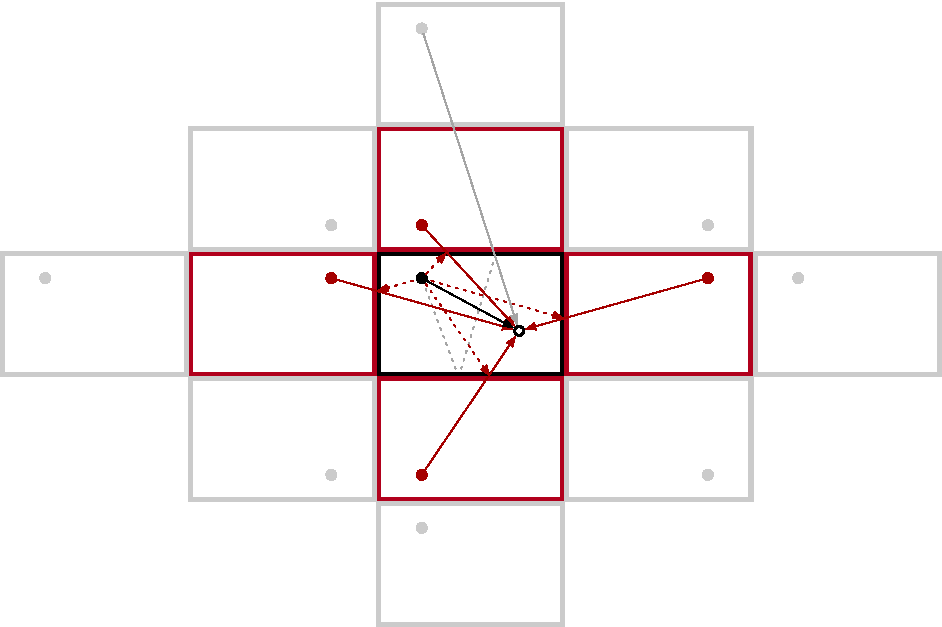
\includegraphics[width=\textwidth]{data/figures/image-method3}
    \caption[Second Order Image Expansion for a Single Source and Receiver]{Second Order Image Expansion for a Single Source and Receiver: \itshape The black rectangle represents the room that is being simulated, containing the source (black dot) and the receiver (black circle). The red rectangles represent the first-order image expansion, where every acoustic wave arriving at the receiver after being reflected one time (dotted red arrows) is simulated as a direct arrival wave (red arrows) to the virtual source (red dot) in the image of the room. The image is created by mirroring the room at the wall where the reflection occured. The grey rectangles represent the second-order images for signal waves that are subject to two reflections (dotted grey arrow).}
    \label{fig:imageMethod}
\end{figure}

To conduct the experimental part of this thesis, simulation as means of data collection has been chosen over real recordings, as simulated acoustic environments are more flexible compared to a laboratory environment. To simulate the experimental setup described in Section \ref{sec:setup}, the \emph{image-source method} for small-room acoustics is used \cite{Allen1979}. The basic idea of this technique is to simulate an arriving signal wave reflected from the walls like a wave arriving directly from virtual sources, mirrored at the reflecting wall. Two parameters determine, how many images are created during simulation with everything else being equal: The reverberation time T$_{60}$, the time it takes the source signal to have decreased by 60dB after the exciting source is switched off, and the reflection order $r$, which is equal to the maximum order of the image expansion. Instead of explicitly stating T$_{60}$, the wall reflection coefficients $\bm\beta = [\beta_1~\beta_2~\dots~\beta_6]$ could also be provided, simulating different types of walls, like concrete walls or walls with soundproofing. There is one coefficient per wall, including the ceiling and the floor, for a total of six coefficients. Whenever the signal crosses a wall into another image (i.e., being reflected), it is attenuated by the $\beta$-coefficient of that wall. An example of a second-order image expansion is shown in \autoref{fig:imageMethod}.

This method allowed for experiments, where a controlled acoustic environment in the form of a small, rectangular room is required that can be easily adjusted. For many experiments, constructing such an environment in a laboratory is prohibitive, which is why the image method has gained widespread popularity since its inception in \citeyear{Allen1979}~\cite{Allen1979} and has been used in a wide range of studies \cite{Champagne1996}.